\documentclass[a4paper,10pt]{scrbook}

\usepackage{amsmath,amsthm,amssymb}
\usepackage{mathenv,textcomp, graphicx}

\begin{document}
This theory is an attempt to model the heat exchange phenomena between a thermally charged fluid and a non-consolidated aggregate material in a non-pressurized, gravitationally charged hydrodynamic environment.

\begin{center}
 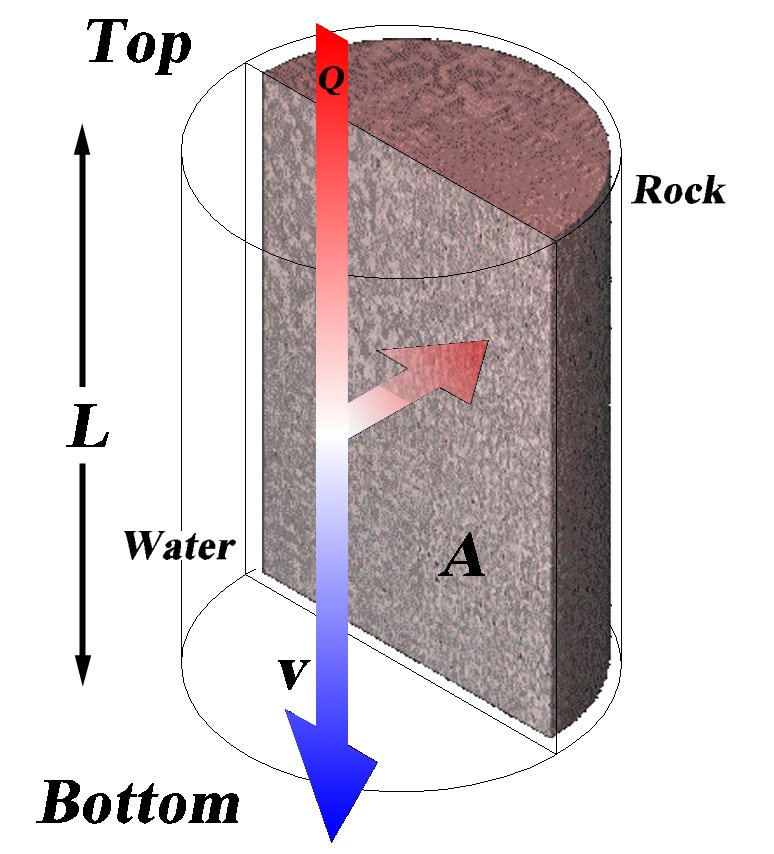
\includegraphics[scale=0.2]{theorySlab.jpg}
 % theorySlab.jpg: 774x854 pixel, 72dpi, 27.31x30.13 cm, bb=0 0 774 854
\end{center}

\begin{equation*}
\begin{split}
\frac{\partial Q(y,t)}{\partial t} &= -k\, \left(\frac{A}{R}\right)\,T_{WR}(y,t)\\
\int_{Q(y,0)}^{Q(y,t_{f})} d\,Q(y,t)\,&=\,-k\,\left(\frac{A}{R}\right)\int_{0}^{t_{f}}\,T_{WR}\,(y,t)\,dt\\
\end{split}
\end{equation*}
$\mathbf{\ni}$\\ 
\textbf{  Which yields the heat lost from 1 vertical ''slab'' over time, }$\mathbf{0\;<\;t\;<\;t_{f}}$ \ldots
\begin{equation*}
Q(y,t_{f})-Q(y,0)=-k\,\left(\frac{A}{R}\right)\;\int_{0}^{t_{f}}\,T_{WR}(y,t)\,dt\\
\end{equation*} 
\textbf{Now, get the total heat lost over entire length,} $\mathbf{0\;<\;y\;<\;L}$
\begin{equation*}
\begin{split}
\int_{0}^{L}\left[Q(y,t_{f})-Q(y,0)\right]\,dy&=-k\left(\frac{A}{R}\right)\,\int_{0}^{t_{f}}\left[\int_{0}^{L}T_{WR}(y,t_{l})dy\right]\,dt\\
\intertext{or\ldots}
L\,\left[Q_{tot}-Q_{0}\right]&=-k\left[\frac{A}{R}\right]\,\int_{0}^{t_{f}}\left[\int_{0}^{L}T_{WR}(y,t)\,dy\right]\,dt\\
\end{split}
\end{equation*}
\textbf{Finally,}
\begin{equation*}
\boxed{ Q_{tot}-Q_{0}=-k \left( \dfrac{A}{R}\right) \int_{0}^{b_{f}} \left[ \dfrac{1}{L} \int_{0}^{L} T_{WR}(y,t) dy \right] dt }\tag{1}
\end{equation*} 
\textbf{Now, consider for a vertical slot over a small time step\ldots}
\begin{equation*}
\begin{split}
Q(y+dt)-Q(y,t)&=C_{N}\left[T_{W}(y,t+dt)-T_{W}(y,t)\right]\;\Rightarrow C_{W}=m_{W}c_{W}
\intertext{and\ldots}
\frac{Q(y+dt)-Q(y,t)}{dt}\;&=\;C_{W}\frac{\left[T_{W}(y,t+dt)-T_{W}(y,t)\right]}{dt}\\
\intertext{or\ldots}\\
\dot{Q}(y,z)&=C_{W}\dot{T}_{W}(y,t)\\
\intertext{or\ldots}
dQ(y,t)&=C_{W}\dot{T}(y,t)dt
\intertext{Integrating\ldots}
\int_{Q(y,0)}^{Q(y,t_{F}}dQ(y,t)&=C_{W}\,\int_{0}^{t_{f}}\dot{T}(y,t)dt\\
Q(y,t_{f})-Q(y,0)&=C_{W}\,\int_{0}^{t_{f}}\dot{T}_{W}(y,t)dt\\
\intertext{Get total heat lost from vessel\ldots}
\end{split}
\end{equation*} 
\begin{equation*}
\boxed{ Q_{tot}-Q_{0}=C_{W}\int_{0}^{t_{f}}\left[\dfrac{1}{L}\int_{0}^{L}\dot{T}_{W}(y,t)dy\right]\,dt}\tag{2}
\end{equation*}
Equate the right hand side of (1) and (2)\ldots
\begin{equation*}
\begin{split}
-k\left(\frac{A}{R}\right)\int_{0}^{t_{f}}\left[\frac{1}{L}\int_{0}^{L}T_{CW}(y,t)dy\right]\;dt\;&=\;C_{W}\int_{0}^{t_{f}}\left[\frac{1}{L}\int_{0}^{L}\dot{T}_{W}(y,t)dy\right]\,dt
\intertext{To be true, the integrands must be equal\ldots}
-k\left(\frac{A}{R}\right)T_{WR}(y,t)&=C_{W}\dot{T}_{W}(y,t)\\
\end{split}
\end{equation*}
\begin{equation*}
\boxed{\dot{T}_{WR}(y,t)=-\frac{kA}{C_{WR}R}T_{WR}(y,t)}\tag{3}
\end{equation*}
Now, to solve this, realize that the rate of heat loss by the water equals the rate of heat gained by the rock\ldots
\begin{equation*}
\begin{split}
\dot{Q}=C_{W}\dot{T}_{W}\text{ and } \dot{Q}_{R}=C_{R}\dot{T}_{R}\\; : \\; C_{R}=m{R}c{R}\\
\intertext{and\ldots}
\dot{Q}_{W}=\dot{Q}_{R}\text{\textrightarrow}\\
\dot{T}_{WR}&=\dot{T}_{W}-\dot{T}_{R}\\
&=\dot{T}_{W}\left(1-\frac{C_{W}}{C_{R}}\right)\\
&=\dot{T}_{W}\left(1-\frac{C_{R}-C_{W}}{C_{R}}\right)\\
\end{split}
\end{equation*} 
\begin{equation*}
\boxed{\dot{T}_{W}=\dot{T}_{WR}\left(\frac{C_{R}-C_{W}}{C_{R}}\right)^{-1}}\tag{4}
\end{equation*} 
\begin{equation*}
\boxed{\dot{T}_{WR}(y,t)=-\frac{kA}{m_{W}c_{W}R}\left(\frac{C_{R}-C_{W}}{C_{R}}\right)T_{WR}(y,t)}\tag{5}
\end{equation*} 
\vspace{1cm}\linebreak
This has the solution:
\begin{equation*}
\boxed{T_{WR}(y,t)=T_{WR}(y,0)e^{-\alpha t}}\tag{6}
\end{equation*}
\vspace{1cm}
\begin{equation*}
\begin{split}
\text{Where  }\alpha=\frac{kA}{m_{W}c_{W}R}\left(\frac{C_{R}-C_{W}}{C_{R}}\right)\\
\boxed{=\frac{kA}{R}\left(\frac{C_{R}-C{W}}{C_{W}C{R}}\right)}
\end{split}\tag{7}
\end{equation*}

And finally,

\begin{equation*}
\boxed{\dot{T}_{WR}(y,t)=(-\alpha)T-{WR}(y,0)e^{-\alpha t)}}\tag{8}
\end{equation*}
\pagebreak
\vspace{0.5cm}\linebreak
Let $T_{WR}(y,0)=T_{WR}(0,0)e(-\beta y)$ to represent the top temperature as a constant.
\vspace{0.5cm}\linebreak
In this case, $\beta \equiv \left(\dfrac{C_{R}C{W}}{C_{R}-C{W}}\right)\dfrac{v}{kAL}$ where $v$ is the flow velocity through the vessel. 
\begin{equation*}
\begin{split}
T_{WR}(y,t)=&T_{WR}(0,0)e^{-\beta y}e^{-\alpha t} \quad\text{\ldots from (6)}\\
\bar{T}_{WR}(t)=&\frac{1}{L}\int_{0}^{L}T_{WR}(0,0)e^{-\beta y}e^{-\alpha t}\,dy\\
=&\frac{1}{\beta L}T_{WR}(0,0)e^{-\alpha t}e^{-\beta y}\vert_{0}^{L}\\
=&\frac{T_{WR}(0,0)}{\beta L}(1-e^{-\beta L}e^{-\alpha t}
\end{split}
\end{equation*}
\vspace{0.5cm}
So now (1) becomes \ldots
\begin{equation*}
\begin{split}
Q_{tot}-Q{0}=&-k\left(\frac{A}{R}\right)\left(\frac{T_{WR}(0,0)}{\beta L}\right)1-e^{-\beta L} \int_{0}^{t_{f}}e^{-\alpha t}\,dt\\
\text{Let }\gamma =&-k\left(\frac{A}{R}\right)\left(\frac{T_{WR}(0,0)}{\beta L}\right)1-e^{-\beta L}\\
\end{split}
\end{equation*}
and so  \centering\boxed{Q_{tot}=Q_{0}-\frac{\gamma}{\alpha}(1-e^{-\alpha t})}     (11)
\vspace{2cm}\linebreak
skipping the check part for now...\linebreak
\vspace{2cm}\linebreak
\begin{equation*}
\begin{split}
Q_{tot}-Q{0}=-C_{W}\left(\frac{C_{R}}{C_{R}-C_{W}}\right)\dfrac{\alpha}{\beta L} T_{WR}(0,0)(1-e{-\beta L})\int_{0}^{t_{f}}e^{-\alpha t}\,dt\\
\intertext{and\ldots}\\
\gamma=C_{W}\left(\frac{C_{R}}{C_{R}-C_{W}}\right)\dfrac{\alpha}{\beta L} T_{WR}(0,0)(1-e{-\beta L})\\
\boxed{Q_{tot}=Q_{0}-\frac{\gamma}{\alpha}(1-e^{-\alpha t})}\\
\intertext{and finally, we can write everything together\ldots}\\
\boxed{\dot{Q}=-\gamma e^{-\alpha t}=-\left(\frac{k^{2}A^{2}(C_{R}-C_{W})}{RvC_{R}C_{W}}\right)T_{top}(1-e^{-\beta L})e^{-\alpha t}}
\end{split}\tag{13}
\end{equation*}

\end{document}
